\documentclass[a4paper]{article}

\usepackage[a4paper,top=2cm,bottom=2cm,left=3cm,right=3cm,marginparwidth=1.75cm]{geometry}
\usepackage[utf8]{inputenc}
\usepackage[T1]{fontenc}
\usepackage{textcomp}
\usepackage[ngerman]{babel}
\usepackage{amsmath, amssymb, nccmath}
\usepackage{accents}


\usepackage{multirow}
\usepackage{fancyhdr}
\usepackage{lastpage}

% figure support
\usepackage{import}
\usepackage{xifthen}
\pdfminorversion=7
\usepackage{pdfpages}
\usepackage{transparent}
\newcommand{\incfig}[1]{%
    \def\svgwidth{\columnwidth}
    \import{./figures/}{#1.pdf_tex}
}

\pdfsuppresswarningpagegroup=1

\title{Protokoll zur ersten Laborübung\\Messtechnik Labor 376.091}
\author{DINC Atilla (11917652)}

\begin{document}
\newcommand{\unit}[1]{\ensuremath{\, \mathrm{#1}}} % Einheiten in Math-Moder richtig formatieren
% --------------------- HEADER ---------------------
\pagestyle{fancy}
% --------------------- FOOTER ---------------------
\fancyfoot[L]{Wintersemester 2023}
\fancyfoot[C]{\textbf{\thepage /\pageref{LastPage}}}
\renewcommand{\footrulewidth}{0.4pt}

\normalsize
\maketitle
\tableofcontents

\begin{center}
	\begin{tabular}{|c| c| c| c| c|}
		\hline
		\multicolumn{5}{|c|}{\textbf{Geräteliste}}                                                                                        \\
		\hline

		Bezeichnung              & Gerätebeschreibung                                         & Messgrößen & Inventarnummer & Bemerkungen \\
		\hline
		MM0                      & Agilent Digitalmultimeter True RMS                                  & -          & U1232A         & -           \\
		MM1                      & Digitalmultimeter                                          & -          & #11            & -           \\
		MM2                      & Digitalmultimeter                                          & -          & #7             & -           \\
		\multirow{2}{*}{OZ1}     &
		\multirow{2}{*}{
			\begin{tabular}[c]
				Digitalspeicheroszilloskop DSO-x2002A \\
				MMSR
			\end{tabular}
		}                        &
		\multirow{2}{*}{-}     &
		\multirow{2}{*}{C0404-5} &
		\multirow{2}{*}{-}                                                                                                                \\
		                         &                                                            &            &                &             \\
		NG1                      & Netzgerät 2-Channel $\pm10\unit{mV}$                       & -   & CD0404-6       & -           \\
		FG1                      & Funktionsgenerator                                         & -    & SDG1025        & -           \\
		\hline
		\hline
		\multicolumn{5}{|c|}{\textbf{Zubehörliste}}                                                                                       \\
		\hline

		Bezeichnung              & Zubehörbeschreibung                                        & Messgrößen & Inventarnummer & Bemerkungen \\
		\hline
		K1                       & Tastkopf (10:1) 100\unit{MHz} 10\unit{M\Omega} 15\unit{pf} & -          & -              & rot         \\
		K2                       & Tastkopf (10:1) 150\unit{MHz} 10\unit{M\Omega} 15\unit{pf} & -          & -              & grau        \\
		K3                       & Tastkopf (10:1) 150\unit{MHz} 10\unit{M\Omega} 15\unit{pf} & -          & -              & rosa        \\
		\hline
	\end{tabular}
\end{center}
\newpage
% ~~~~~~~~~~~~~~~~~~~~~~~~~~~~ Start of the document ~~~~~~~~~~~~~~~~~~~~~~~~~~~~

\section{Einleitung}

\section{Messungen mit dem Digitalmultimeter}
\subsection{Spannungsmessung}
Zur Spannungsmessung wird der Spannungseingang des Multimeters parallel zur Messgröße
geschaltet, daher ist ein möglichst hoher Innenwiderstand $R_{i}$ erwünscht. Zur
Bestimmung dieses Innenwiderstands $R_{i}$ sollte eine Serienschaltung mit einem 
relativ hochohmigen bekannten Widerstand aufgebaut und der Spannungsabfall am Multimeter
von diesem abgelesen werden.\newline
Weiters sollte der Einfluss des Multimeters auf die Schaltung gemessen werden,
indem der Spannungseingang eines Multimeters des gleichen Models parallel zum 
Multimeter angeschlossen wird. \newline
Zuletzt sollte eine Messbereichserweiterung durchgeführt werden, indem ein
Serienwiderstand bekannter Größe in den Strompfad verbaut und der 
Spannungsabfall gemessen wird gemessen wird.

\subsubsection{Messaufbau und Messdurchführung}
\subsubsection*{Bestimmung des Innenwiderstandes}
Die eingestellte Spannung des Netzgerätes FG1 wurde mit dem Multimeter MM0 
geprüft bevor sie mit der Schaltung belastet wurde. Der Serienwiderstand R1 wurde
mit dem Multimeter MM0 bestimmt.
Im Anschluss wurde die Schaltung wie in Abb. \ref{fig:RiVM} angeschlossen.
Die angezeigte Spannung am Multimeter MM1 wurde abgelesen und die Eingangsspannung
wurde erneut gemessen. Weder die Eingangsspannung, noch die Spannung am Multimeter
MM1 haben sich geändert. Somit wurde sichergestellt, dass sowohl Innenwiderstand
des Netzgerätes, als auch jegliche Kontaktwiderstände in der Schaltung
vernachlässigbar klein für unsere Messungen waren.\newline
Der Kontrollprozess wurde vor allen folgenden Messungen durchgeführt, um die
Eingangsspannung möglichst genau zu bestimmen.
\begin{figure}[h]
    \centering
    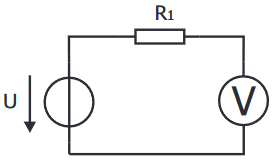
\includegraphics[width=0.4\textwidth]{schematics/1a_RiVM.png}
    \caption{Schaltung zur Bestimmung des Multimeter-Innenwiderstands}
    \label{fig:RiVM}
\end{figure}

\subsubsection*{Bestimmung des Einflusses}
Für diese Messung wurde die Eingangsspannung $U_{q}$ wie zuvor gemessen.
Als Widerstand $R_{M}$ wurde der gleiche Widerstand wie zuvor verwendet und auch
und auch das Multimeter MM1 wurde nicht gewechselt, somit konnte die vorherige
Schaltung beibehalten und wie in Abbildung \ref{fig:1b_EinflussVM} erweitert werden.
Die Spannungen an den Multimetern wurden zunächst mit nur einem Multimeter MM1
und danach mit beiden Multimetern MM1 und MM2 abgelesen.
\begin{figure}[h]
    \centering
    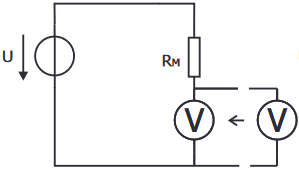
\includegraphics[width=0.4\textwidth]{schematics/1b_EinflussVM.png}
    \caption{Schaltung zur Bestimmung des Einflusses}
    \label{fig:1b_EinflussVM}
\end{figure}

\subsubsection*{Messbereichserweiterung}
Zur Messbereichserweiterung wurde die Schaltung wie in Abb. \ref{fig:1c_MB-ErweiterungVM}
aufgebaut. Dabei wurde der Widerstand $R_{M}$ aus der vorherigen Schaltung
und zur Messbereichserweiterung verwendet. Die zu messenden Spannungen in dieser
Schaltung liegt am Widerstand $R_{V}$ an und soll in etwa halbiert werden, indem
die Widerstände mit $R_{M}\approx R_{V}$ auch in etwa gleich groß gewählt werden.

\begin{figure}[h]
    \centering
    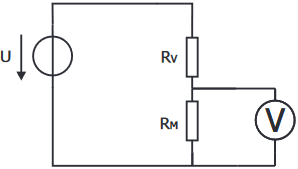
\includegraphics[width=0.4\textwidth]{schematics/1c_MessbereichserweiterungVM.png}
    \caption{Schaltung zur Messbereichserweiterung eines Voltmeters}
    \label{fig:1c_MB-ErweiterungVM}
\end{figure}


\subsubsection{Messergebnisse}
\subsubsection*{\textbf{Bestimmung des Innenwiderstandes}}
Die Schaltung wurde mit einer gemessenen Eingangsspannung $U_{q}=9,92\unit{V}$ und einem
gemessenen Widerstand $R_{1}=98,9 \unit{k\Omega}$ aufgebaut. Weiters wurde am
Multimeter MM2 die Spannung $U_{V}=9,84\unit{V}$ gemessen. Mithilfe der Formel
für den Spannungsteiler kann die Gleichung
\[ U_{V}=U_{q} \frac{R_{i}}{R_{1}+R_{i}} = U_{q} \frac{1}{1 + \frac{R_{1}}{R_{i}}}\]
aufgestellt werden, woraus sich direkt durch Umformung
    \[ R_{i}=\frac{R_{1}}{\frac{U_{q}}{U_{v}}-1} \]
ergibt.
Wir errechnen also einen Innenwiderstand $R_{i}\approx 12,1647 \unit{M\Omega}$.

\subsubsection*{\textbf{Bestimmung des Einlusses}}

\subsection{Strommessung}
Ähnlich zur Messung mit einem Voltmeter wird auch bei einer Strommessung die
Schaltung durch das Amperemeter belastet. Da die ein Amperemeter seriell zum
stromdurchflossenen Bauteil verschaltet wird, muss der Innenwiderstand möglichst
klein sein, um möglichst keinen Spannungsabfall zu verursachen.
Kurzbeschreibung hier \ref{fig:EinlussVM}
\begin{figure}[h]
	\centering
	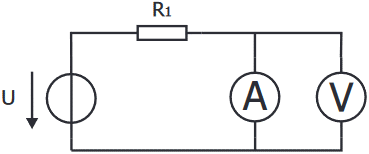
\includegraphics[width=0.8\textwidth]{schematics/2a_RiAM.png}
	\caption{Schaltung zur Messung des Einflusses durch die Messung}
	\label{fig:WUT}
\end{figure}

\subsection{Widerstandsmessung}
\ref{fig:MB-Erweiterung}
\begin{figure}[h]
	\centering
	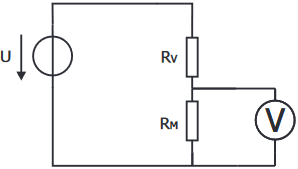
\includegraphics[width=0.8\textwidth]{schematics/1c_MessbereichserweiterungVM.png}
	\caption{Schaltung zur Messbereichserweiterten Messung}
	\label{fig:MB-Erweiterung}
\end{figure}

\section{Messungen mit dem Oszilloskop}
\subsection{Tastkopf}
\subsection{AC-Spannungsmessung}
\subsection{RMS im Detail}
\subsection{Amplitudenauflösung}
\subsection{Dynamik}


\end{document}
